% Chapter Template

\chapter{Development and Discussion} % Main chapter title

\label{Chapter4} % Change X to a consecutive number; for referencing this chapter elsewhere, use \ref{ChapterX}

%----------------------------------------------------------------------------------------
%	SECTION 1
%----------------------------------------------------------------------------------------

\section{Overview}

The first revision of the prototype case is presented in this chapter. 
Specifically, this section goes into detail about the process of designing as an iterative process where improvements and changes to the design are discussed and evaluated.


%----------------------------------------------------------------------------------------
%	SECTION 2
%----------------------------------------------------------------------------------------

\section{Initial Concepts}

At the initial stage of planning, multiple approaches to the MEGAphone chassis were conceptualised before making a final selection. 
Two of these designs incorporated ‘stands’ to prop the device up in order to minimise physical effort from the user, as well as all designs featuring a curved design to accommodate comfortable device holding for a large range of hand grip sizes. 
Each of these designs are outlined in the following sub-sections.

%-----------------------------------
%	SUBSECTION 1
%-----------------------------------
\subsection{Design One}

% LIST PROS AND CONS OF EACH DESIGN
% PERHAPS RANKING SYSTEM, EXPLAIN WHY DESIGN 3 WAS CHOSEN

Design ‘One’ as named was the first concept to be sketched using LibreCAD software. 
In hindsight, most of this design’s features are quite mundane in that while they account for all major ports and include a device stand to prop it up, in terms of the ergonomics, there are very few stand-out features. 
One thing that can be noted is that the case is compact with curved profile on either side where the user’s hands are expected to rest.

% \begin{figure}[hbt!]
% \centering
% 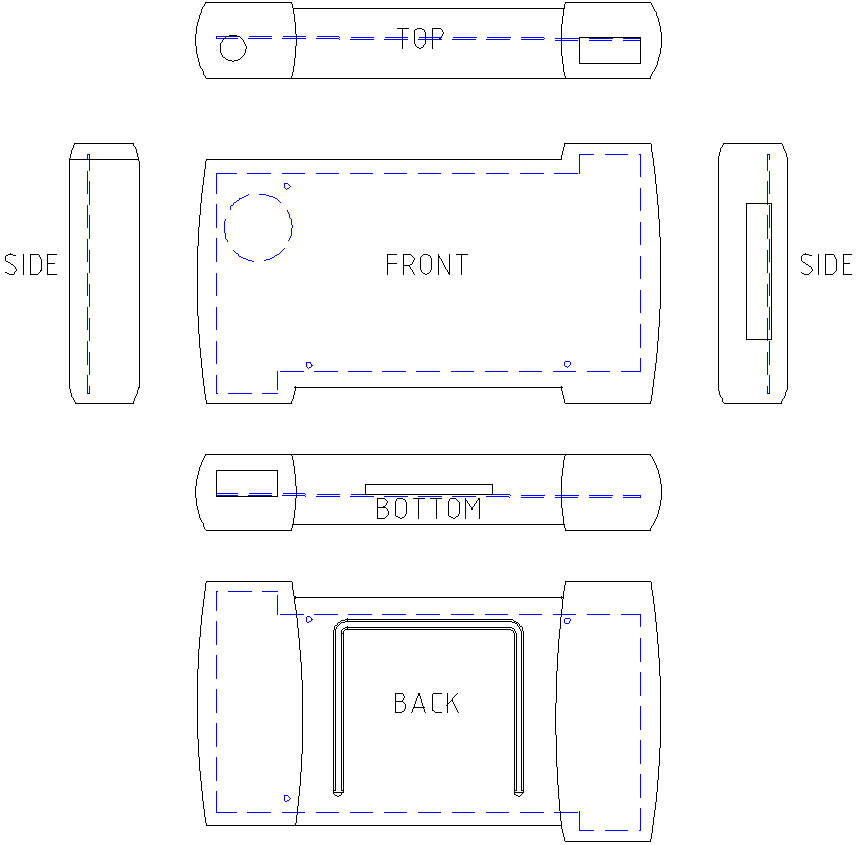
\includegraphics[width=10cm,height=10cm,keepaspectratio]{Figures/design1_sketch.png}
% \caption{This is a sketch of the first concept design drawn to scale of the PCB}
% \label{fig:Design_1}
% \end{figure}

%-----------------------------------
%	SUBSECTION 2
%-----------------------------------
\subsection{Design Two}

The second design was intended to mimic a video game controller in order to conform better to the hand as well as give users a more intuitive layout in regards to the orientation of the device when in use. 
UD and the MEGAphone project have two common traits in that they intend for the device to be simple, to use and to defend against security threats under the mantra ‘security through simplicity’ REF. 
This concept inhabits this trait arguably to the highest degree.

% \begin{figure}[hbt!]
% \centering
% 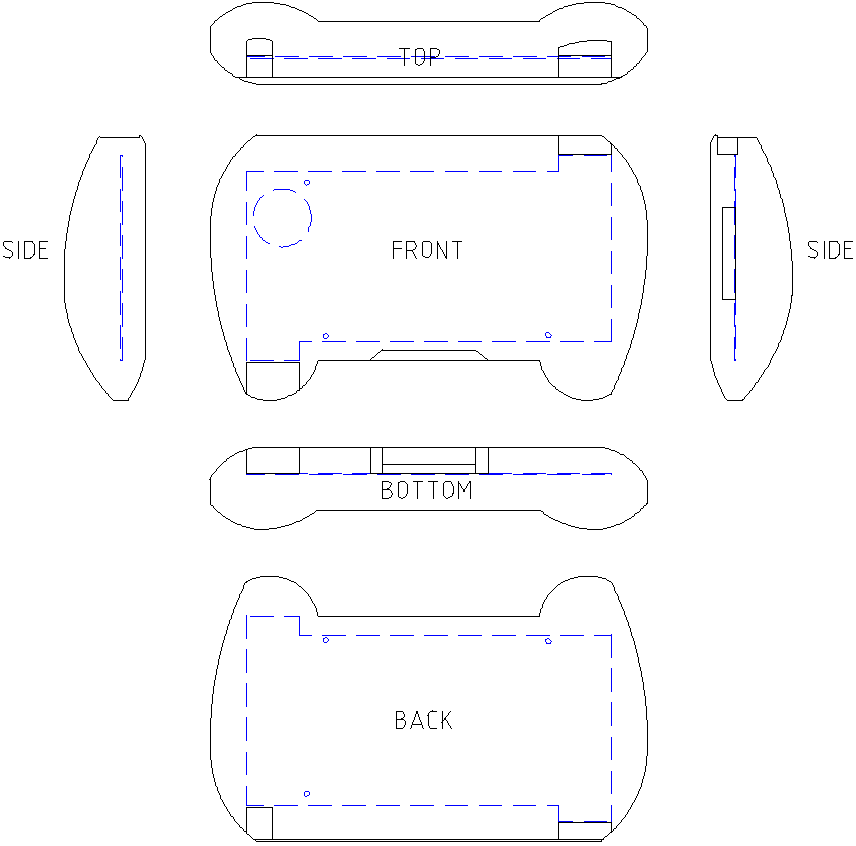
\includegraphics[width=10cm,height=10cm,keepaspectratio]{Figures/design2_sketch.png}
% \caption{This is a sketch of the second concept design drawn to scale of the PCB}
% \label{fig:Design_2}
% \end{figure}

%-----------------------------------
%	SUBSECTION 3
%-----------------------------------
\subsection{Design Three}

There were a few factors that made this design the final candidate in which to base the main deliverable of this project.
This approach uses handgrips to subconciously hint to the user the correct orientation to hold the device.
The use of a stand to prop the device up for extended periods of time was a useful addition as it reduces the amount of effort from the user, therefore reducing fatigue.

% \begin{figure}[hbt!]
% \centering
% 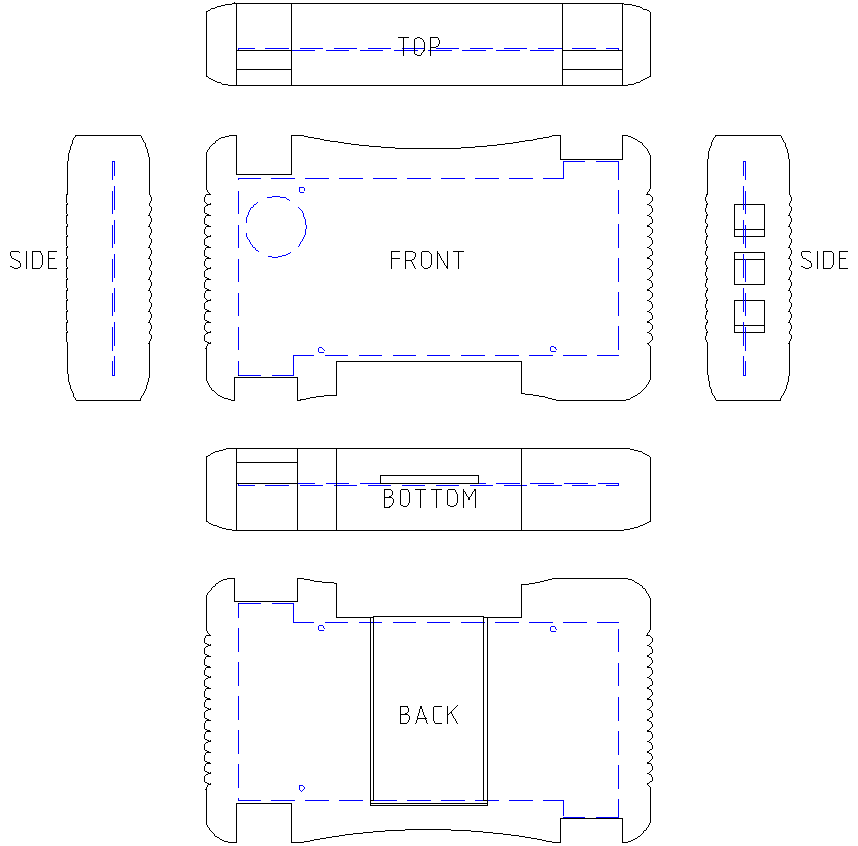
\includegraphics[width=10cm,height=10cm,keepaspectratio]{Figures/design3_sketch.png}
% \caption{This is a sketch of the third concept design drawn to scale of the PCB}
% \label{fig:Design_3}
% \end{figure}

%----------------------------------------------------------------------------------------
%	SECTION 3
%----------------------------------------------------------------------------------------

\section{First Revision}

The following section covers the development of all aspects of the accessible MEGAphone chassis as well as the accompanying hardware such as buttons or hinges.

%-----------------------------------
%	SUBSECTION 1
%-----------------------------------
\subsection{CAD Sketch}

Nunc posuere quam at lectus tristique eu ultrices augue venenatis.

%-----------------------------------
%	SUBSECTION 2
%-----------------------------------
\subsection{Hand Grips}

The first stage of design after the initial concept sketches intended to use rubber grips on both sides of the device, however this concept was removed in favour of a ridges that resemble the size and shape of human adult fingers to more intuitively direct the user to hold the device in the correct fashion. 

% This was after receiving feedback from my supervisor following an initial design (show design, before and after).

%-----------------------------------
%	SUBSECTION 3
%-----------------------------------
\subsection{Rocker Switches}

% placement of switches not very easy to access, so explain why larger rocker switches were chosen, explain the intention behind the orientation of switches; for easier access for those with limited motor function or even without fingers, would ensure less likely to flip wrong switch if rocker sits vertical while switches sit horizontal

%-----------------------------------
%	SUBSECTION 4
%-----------------------------------
\subsection{Jellybean Switch}

The Jellybean switch bought exclusively for this project interfaces with the device using a 3.5mm Audio Jack connector. 
Given that it is a single digital input device, hardware-implemented software accessibility capable of easily communicating with this device was relatively simple to implement. 
The second revision PCB during commencement of this project did not feature a working 3.5mm Jack connector, therefore, based on this knowledge, the 9-pin DSUB port of the device was hijacked as a single digital input under pin 7 for the Jellybean switch. 
The PCB ‘adapter’ created for this purpose is discussed in \section{4.3}.
This uses the same pin as the fire button on a retro Commodore64 Joystick controller, hence, integration into the MEGA65 operating system would be straightforward.

%-----------------------------------
%	SUBSECTION 5
%-----------------------------------
\subsection{Recessed Buttons}

% talk about recessing the buttons so that if the device is dropped, minimal/no accidental button presses are registered

One concept that would improve the ‘quality of life’ of this product was the addition of recessed buttons. 
There are potential situations where the device might be accidentally dropped and unintended button presses may be recorded. 
Recessed buttons reduce the likeliness of this situation

%-----------------------------------
%	SUBSECTION 6
%-----------------------------------
\subsection{3D-printed Prototype}

talk about how 3D printed prototype was not correct; the thought behind orientation of components was flipped and therefore does not fit in case, ports/components need more space in order to fit comfortably, so explain the process of rectifying this issue, map out the impacts and how they are resolved
also add in that 0.15mm print resolution was not suitable as the project was very precise on top case in some parts, such as buttons, hence this should be done at higher resolution which means longer print time or silicone injection mould as a likely stronger, neater alternative

%-----------------------------------
%	SUBSECTION 7
%-----------------------------------
\subsection{Solar Panels}

choice of solar panels, discuss potential options and why a specific one was chosen, do a table comparison of available panels and again explain the power output and cost etc.

%-----------------------------------
%	SUBSECTION 8
%-----------------------------------
\subsection{Device Stand}

thoughts behind the device stands, how they were conceptualised and why it was approached in such and such way; having two stands on either side adds to stability of the device as opposed to the original idea of having one stand in the middle, which also leaves space for solar panel in the middle

%-----------------------------------
%	SUBSECTION 9
%-----------------------------------
\subsection{Device Strap / Key-chain}

% talk about process of designing this feature, how original design changed in favour of larger slot/strap for easier carry

%-----------------------------------
%	SUBSECTION 10
%-----------------------------------
\subsection{Easy Access Keys}

Nunc posuere quam at lectus tristique eu ultrices augue venenatis.
% FIXED AB AND DIRECTIONAL BUTTON SIZE CLEARANCE, ALSO EZ KEY CLEARANCE
% FIXED ALIGNMENT OF THROUGH HOLE

%-----------------------------------
%	SUBSECTION 11
%-----------------------------------
\subsection{Ventilation}

device only uses about 1-2W of power, FPGA using 0.2W
Not necessary in final design but add images of version with vents

%-----------------------------------
%	SUBSECTION 12
%-----------------------------------
\subsection{Potentiometers}

Slide pot better than thumb wheel pot, explain about physical effort etc.


%----------------------------------------------------------------------------------------
%	SECTION 4
%----------------------------------------------------------------------------------------

\section{PCB Design}

% explain workaround for previous button layout, using slave boards with tactile switches as well as choice behind contact pads instead of connectors to save space

%-----------------------------------
%	SUBSECTION 1
%-----------------------------------
\subsection{Rocker Switch PCB}

Nunc posuere quam at lectus tristique eu ultrices augue venenatis.

%-----------------------------------
%	SUBSECTION 2
%-----------------------------------
\subsection{Easy Keys and Power}

Nunc posuere quam at lectus tristique eu ultrices augue venenatis.

%-----------------------------------
%	SUBSECTION 3
%-----------------------------------
\subsection{Audio Jack Adapter}

Nunc posuere quam at lectus tristique eu ultrices augue venenatis.


%----------------------------------------------------------------------------------------
%	SECTION 5
%----------------------------------------------------------------------------------------

\section{PCB Layout}

% analyse the changes in the final design, what limitations the existing PCB layout has and propose a better layout that satisfies the UD principles, talk about what is ideal and what is the best that can be done with current layout. 
% Ideal layout includes ports at top of device along with rocker switches replacing current rev2 switches on the main PCB

%-----------------------------------
%	SUBSECTION 1
%-----------------------------------
\subsection{Original Design}

The layout of the second revision MEGAphone PCB served as the major constraint of this project, as the case design had to be designed around it without any significant redesign due to the complexity of the device. Certain reworks to better adapt the design to an accessible interface included removing the existing switches in favour of larger rocker switches hosted on an external PCB (VIEW).

%-----------------------------------
%	SUBSECTION 2
%-----------------------------------
\subsection{Proposed Design}

A possible solution to the existing PCB which does inhabit the Universal Design principles is proposed in FIGURE. 
The underlying idea with this redesign was to integrate the design all onto one PCB. Doing so would reduce the amount of wires required and given that those in the current solution are soldered to make space, it makes the design overall ‘simpler’.

In order to make the device more intuitive, placement of the 9-pin DSUB port should be moved to the ‘top’ of the device in the same orientation as the VGA port, so that users know from a glance that this is where all device ports are expected to be.
The accessible button interface also utilises an external PCB which hosts the tactile switches that were opted to form the base of the accessible button function. 
Other options were considered, such as silicone rubber pads, as used for the directional button and ‘A’, ‘B’ buttons. However, due to the nature of the


%----------------------------------------------------------------------------------------
%	SECTION 6
%----------------------------------------------------------------------------------------

\section{Software}

talk about keyboard accessibility, term ‘android accessibility encapsulation’ discuss this. 
Also mention program is working in parallel to the software ‘mimicking’ the c64 system so this is not a C program running on MEGA65 but rather VDHL, a hardware description language

%-----------------------------------
%	SUBSECTION 1
%-----------------------------------
\subsection{Accessible Keyboard}

Nunc posuere quam at lectus tristique eu ultrices augue venenatis.

%-----------------------------------
%	SUBSECTION 2
%-----------------------------------
\subsection{PART2}

Nunc posuere quam at lectus tristique eu ultrices augue venenatis.

%-----------------------------------
%	SUBSECTION 3
%-----------------------------------
\subsection{PART3}

Nunc posuere quam at lectus tristique eu ultrices augue venenatis.

%----------------------------------------------------------------------------------------
%	SECTION 7
%----------------------------------------------------------------------------------------

\section{Summary}

Lorem ipsum dolor sit amet, consectetur adipiscing elit.